% pdflatex map_sheet.tex
% TODO: add this to the Makefile.
\documentclass[parskip]{scrartcl}
\usepackage{graphicx,overpic}
% Consider making margins either 0 or 0.1in.
\usepackage[paperheight=17in,paperwidth=11in,margin=0.25in]{geometry}

\usepackage{geometry}
\usepackage{multicol}
\usepackage{amsmath}
\usepackage{titlesec}
\usepackage{diagbox,pict2e}
\usepackage{makecell}
\usepackage{tabularx}
\usepackage{multirow}
\usepackage{lscape}
\usepackage{tikz}
\usepackage{adjustbox}


\begin{document}

\begin{center}
  \begin{overpic}[width=10.5in, grid=false]{map.pdf}

    \put(10, -100){\includegraphics[width=9in]{../rules/nv-air-status.pdf}}


    % Victory Points Track (PDF from ../rules/)
    % \put(20, 85){\includegraphics[width=5in]{../rules/victory-points.pdf}}

    \put(5, -65){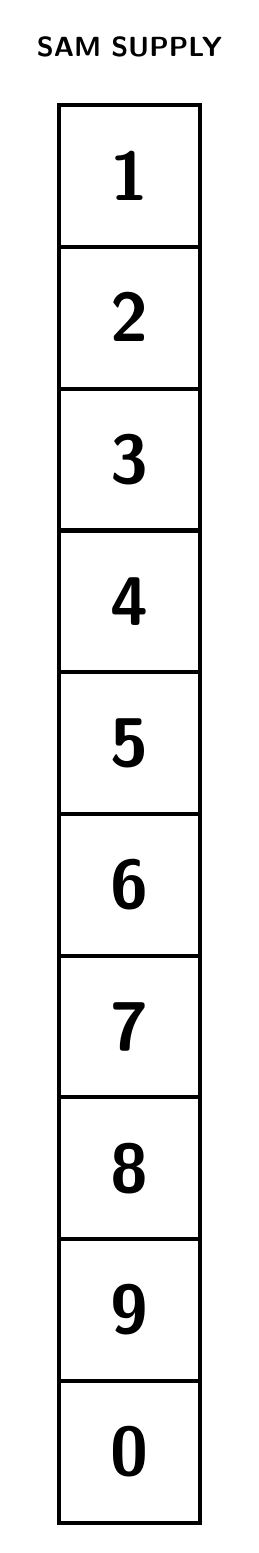
\begin{tikzpicture}
    % Define box properties
    \def\boxwidth{1.8}
    \def\boxheight{1.8}
    \def\boxthickness{1.5pt} % Adjustable line thickness

    % Define SAM Supply numbers (1 to 0)
    \def\samsupply{1, 2, 3, 4, 5, 6, 7, 8, 9, 0}

    % Title at the top
    \node[anchor=south] at (0.9, 0.5) {\sffamily \bfseries SAM SUPPLY};

    % Draw boxes and numbers
    \foreach \x [count=\i] in \samsupply {
        \pgfmathsetmacro\ypos{-(\i-1) * \boxheight} % Calculate vertical position
        \draw[line width=\boxthickness] (0, \ypos) rectangle (\boxwidth, \ypos - \boxheight);
        \node at (0.9, \ypos - 0.9) {\sffamily \bfseries \Huge \x}; % Centered inside box
    }

\end{tikzpicture}
}
    \put(90, -55){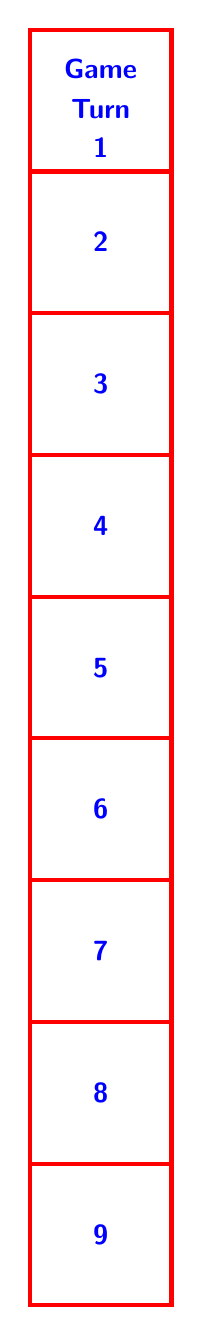
\begin{tikzpicture}

  % Define the gray color matching SVG default gray
  \definecolor{svggray}{RGB}{128,128,128}
  
  % Apply to everything
  \tikzset{every picture/.style={color=red}}

  \tikzset{every node/.style={text=blue}, every path/.style={draw=red}}


    % Define box properties
    \def\boxwidth{1.8}
    \def\boxheight{1.8}
    \def\boxthickness{1.5pt} % Adjustable line thickness

    % Define Game Turn numbers (2 to 9, since 1 is in the title box)
    \def\gameturns{2, 3, 4, 5, 6, 7, 8, 9}

    % First box with "Game Turn 1"
    \draw[line width=\boxthickness] (0, 0) rectangle (\boxwidth, -\boxheight);
    \node at (0.9, -0.5) {\sffamily \bfseries Game};
    \node at (0.9, -1.0) {\sffamily \bfseries Turn};
    \node at (0.9, -1.5) {\sffamily \bfseries 1};

    % Draw boxes and numbers for turns 2-9
    \foreach \x [count=\i] in \gameturns {
        \pgfmathsetmacro\ypos{-\i * \boxheight} % Calculate vertical position
        \draw[line width=\boxthickness] (0, \ypos) rectangle (\boxwidth, \ypos - \boxheight);
        \node at (0.9, \ypos - 0.9) {\sffamily \bfseries \x}; % Centered inside box
    }
\end{tikzpicture}
}
    \put(10, -75){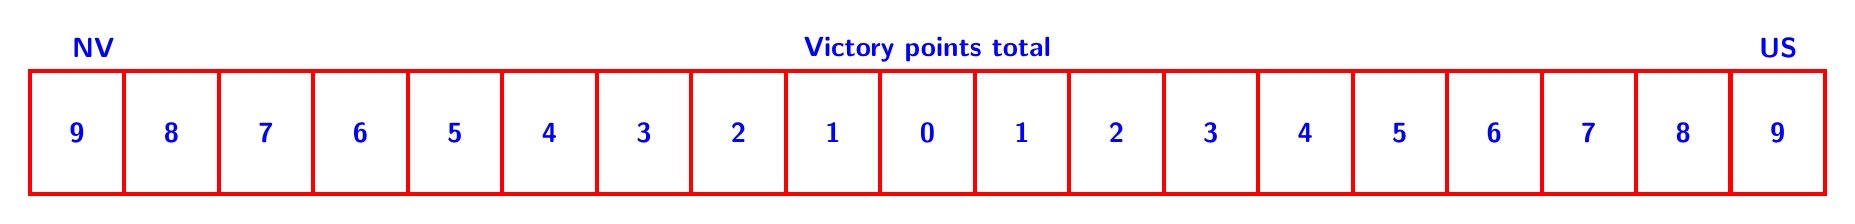
\begin{tikzpicture}[scale=1.2]
    \tikzset{every node/.style={text=blue}, every path/.style={draw=red}}

    % Define box size
    \def\boxwidth{1.0}
    \def\boxheight{1.3}
    \def\boxthickness{1.5pt} % Parameterized line thickness

    % Define victory points (NV decreasing, US increasing)
    \def\victorypoints{9, 8, 7, 6, 5, 4, 3, 2, 1, 0, 1, 2, 3, 4, 5, 6, 7, 8, 9}

    \def\ypos{0.25}
    % Labels
    \node[anchor=east] at (1, \ypos) {\sffamily \bfseries NV};
    \node[anchor=west] at (18*\boxwidth + 0.2, \ypos) {\sffamily \bfseries US};
    \node[anchor=south] at (9.5*\boxwidth, \ypos-0.25) {\sffamily \bfseries Victory points total}; % Centered over the track

    % Draw boxes and numbers
    \foreach \x [count=\i] in \victorypoints {
        \pgfmathsetmacro\xpos{\i - 1}
        \draw[line width=\boxthickness] (\xpos*\boxwidth, 0) rectangle (\xpos*\boxwidth + \boxwidth, -\boxheight);
        \node at (\xpos*\boxwidth + 0.5, -0.65) {\sffamily \bfseries \x};
    }

\end{tikzpicture}
}

    % Any additional elements can be positioned here as needed

  \end{overpic}
\end{center}


\end{document}
